% Options for packages loaded elsewhere
\PassOptionsToPackage{unicode}{hyperref}
\PassOptionsToPackage{hyphens}{url}
%
\documentclass[
]{book}
\usepackage{amsmath,amssymb}
\usepackage{lmodern}
\usepackage{iftex}
\ifPDFTeX
  \usepackage[T1]{fontenc}
  \usepackage[utf8]{inputenc}
  \usepackage{textcomp} % provide euro and other symbols
\else % if luatex or xetex
  \usepackage{unicode-math}
  \defaultfontfeatures{Scale=MatchLowercase}
  \defaultfontfeatures[\rmfamily]{Ligatures=TeX,Scale=1}
\fi
% Use upquote if available, for straight quotes in verbatim environments
\IfFileExists{upquote.sty}{\usepackage{upquote}}{}
\IfFileExists{microtype.sty}{% use microtype if available
  \usepackage[]{microtype}
  \UseMicrotypeSet[protrusion]{basicmath} % disable protrusion for tt fonts
}{}
\makeatletter
\@ifundefined{KOMAClassName}{% if non-KOMA class
  \IfFileExists{parskip.sty}{%
    \usepackage{parskip}
  }{% else
    \setlength{\parindent}{0pt}
    \setlength{\parskip}{6pt plus 2pt minus 1pt}}
}{% if KOMA class
  \KOMAoptions{parskip=half}}
\makeatother
\usepackage{xcolor}
\IfFileExists{xurl.sty}{\usepackage{xurl}}{} % add URL line breaks if available
\IfFileExists{bookmark.sty}{\usepackage{bookmark}}{\usepackage{hyperref}}
\hypersetup{
  pdftitle={Comandos básicos do R: Guia de bolso},
  pdfauthor={Lucas C. Germano},
  hidelinks,
  pdfcreator={LaTeX via pandoc}}
\urlstyle{same} % disable monospaced font for URLs
\usepackage{color}
\usepackage{fancyvrb}
\newcommand{\VerbBar}{|}
\newcommand{\VERB}{\Verb[commandchars=\\\{\}]}
\DefineVerbatimEnvironment{Highlighting}{Verbatim}{commandchars=\\\{\}}
% Add ',fontsize=\small' for more characters per line
\usepackage{framed}
\definecolor{shadecolor}{RGB}{248,248,248}
\newenvironment{Shaded}{\begin{snugshade}}{\end{snugshade}}
\newcommand{\AlertTok}[1]{\textcolor[rgb]{0.94,0.16,0.16}{#1}}
\newcommand{\AnnotationTok}[1]{\textcolor[rgb]{0.56,0.35,0.01}{\textbf{\textit{#1}}}}
\newcommand{\AttributeTok}[1]{\textcolor[rgb]{0.77,0.63,0.00}{#1}}
\newcommand{\BaseNTok}[1]{\textcolor[rgb]{0.00,0.00,0.81}{#1}}
\newcommand{\BuiltInTok}[1]{#1}
\newcommand{\CharTok}[1]{\textcolor[rgb]{0.31,0.60,0.02}{#1}}
\newcommand{\CommentTok}[1]{\textcolor[rgb]{0.56,0.35,0.01}{\textit{#1}}}
\newcommand{\CommentVarTok}[1]{\textcolor[rgb]{0.56,0.35,0.01}{\textbf{\textit{#1}}}}
\newcommand{\ConstantTok}[1]{\textcolor[rgb]{0.00,0.00,0.00}{#1}}
\newcommand{\ControlFlowTok}[1]{\textcolor[rgb]{0.13,0.29,0.53}{\textbf{#1}}}
\newcommand{\DataTypeTok}[1]{\textcolor[rgb]{0.13,0.29,0.53}{#1}}
\newcommand{\DecValTok}[1]{\textcolor[rgb]{0.00,0.00,0.81}{#1}}
\newcommand{\DocumentationTok}[1]{\textcolor[rgb]{0.56,0.35,0.01}{\textbf{\textit{#1}}}}
\newcommand{\ErrorTok}[1]{\textcolor[rgb]{0.64,0.00,0.00}{\textbf{#1}}}
\newcommand{\ExtensionTok}[1]{#1}
\newcommand{\FloatTok}[1]{\textcolor[rgb]{0.00,0.00,0.81}{#1}}
\newcommand{\FunctionTok}[1]{\textcolor[rgb]{0.00,0.00,0.00}{#1}}
\newcommand{\ImportTok}[1]{#1}
\newcommand{\InformationTok}[1]{\textcolor[rgb]{0.56,0.35,0.01}{\textbf{\textit{#1}}}}
\newcommand{\KeywordTok}[1]{\textcolor[rgb]{0.13,0.29,0.53}{\textbf{#1}}}
\newcommand{\NormalTok}[1]{#1}
\newcommand{\OperatorTok}[1]{\textcolor[rgb]{0.81,0.36,0.00}{\textbf{#1}}}
\newcommand{\OtherTok}[1]{\textcolor[rgb]{0.56,0.35,0.01}{#1}}
\newcommand{\PreprocessorTok}[1]{\textcolor[rgb]{0.56,0.35,0.01}{\textit{#1}}}
\newcommand{\RegionMarkerTok}[1]{#1}
\newcommand{\SpecialCharTok}[1]{\textcolor[rgb]{0.00,0.00,0.00}{#1}}
\newcommand{\SpecialStringTok}[1]{\textcolor[rgb]{0.31,0.60,0.02}{#1}}
\newcommand{\StringTok}[1]{\textcolor[rgb]{0.31,0.60,0.02}{#1}}
\newcommand{\VariableTok}[1]{\textcolor[rgb]{0.00,0.00,0.00}{#1}}
\newcommand{\VerbatimStringTok}[1]{\textcolor[rgb]{0.31,0.60,0.02}{#1}}
\newcommand{\WarningTok}[1]{\textcolor[rgb]{0.56,0.35,0.01}{\textbf{\textit{#1}}}}
\usepackage{longtable,booktabs,array}
\usepackage{calc} % for calculating minipage widths
% Correct order of tables after \paragraph or \subparagraph
\usepackage{etoolbox}
\makeatletter
\patchcmd\longtable{\par}{\if@noskipsec\mbox{}\fi\par}{}{}
\makeatother
% Allow footnotes in longtable head/foot
\IfFileExists{footnotehyper.sty}{\usepackage{footnotehyper}}{\usepackage{footnote}}
\makesavenoteenv{longtable}
\usepackage{graphicx}
\makeatletter
\def\maxwidth{\ifdim\Gin@nat@width>\linewidth\linewidth\else\Gin@nat@width\fi}
\def\maxheight{\ifdim\Gin@nat@height>\textheight\textheight\else\Gin@nat@height\fi}
\makeatother
% Scale images if necessary, so that they will not overflow the page
% margins by default, and it is still possible to overwrite the defaults
% using explicit options in \includegraphics[width, height, ...]{}
\setkeys{Gin}{width=\maxwidth,height=\maxheight,keepaspectratio}
% Set default figure placement to htbp
\makeatletter
\def\fps@figure{htbp}
\makeatother
\setlength{\emergencystretch}{3em} % prevent overfull lines
\providecommand{\tightlist}{%
  \setlength{\itemsep}{0pt}\setlength{\parskip}{0pt}}
\setcounter{secnumdepth}{5}
\usepackage{booktabs}
\ifLuaTeX
  \usepackage{selnolig}  % disable illegal ligatures
\fi
\usepackage[]{natbib}
\bibliographystyle{plainnat}

\title{Comandos básicos do R: Guia de bolso}
\author{Lucas C. Germano}
\date{2022-05-20}

\usepackage{amsthm}
\newtheorem{theorem}{Theorem}[chapter]
\newtheorem{lemma}{Lemma}[chapter]
\newtheorem{corollary}{Corollary}[chapter]
\newtheorem{proposition}{Proposition}[chapter]
\newtheorem{conjecture}{Conjecture}[chapter]
\theoremstyle{definition}
\newtheorem{definition}{Definition}[chapter]
\theoremstyle{definition}
\newtheorem{example}{Example}[chapter]
\theoremstyle{definition}
\newtheorem{exercise}{Exercise}[chapter]
\theoremstyle{definition}
\newtheorem{hypothesis}{Hypothesis}[chapter]
\theoremstyle{remark}
\newtheorem*{remark}{Remark}
\newtheorem*{solution}{Solution}
\begin{document}
\maketitle

{
\setcounter{tocdepth}{1}
\tableofcontents
}
\hypertarget{sobre-este-livro}{%
\chapter*{Sobre este livro}\label{sobre-este-livro}}
\addcontentsline{toc}{chapter}{Sobre este livro}

Sejam bem-vindos!\\
O objetivo deste livro é disponibilizar para consulta anotações de códigos R de forma prática e rápida. Não há explicações aprofundadas nem se pretende esgotar as possibilidades do conteúdo apresentado, assim, esta documentação deve ser utilizada somente como um guia rápido, pois não passa de um conjunto de rascunhos apreendidos no dia-a-dia da manipulação de dados e na apresentação de resultados. O conteúdo poderá ser baixado nos formatos \texttt{.pdf} ou \texttt{epub}, mas a proposta é que o conteúdo seja dinâmico, com atualizações semanais. A estrutura de construção está disponível no \href{https://github.com/lucascgmermano/guia_de_bolso.git}{GitHub}.\\
Críticas, sugestões ou contribuições de código e conteúdo podem ser enviadas para \url{lucascgermano@gmail.com}. Ficarei muito feliz, qualquer que seja o motivo do contato.

\hypertarget{leitura-de-arquivos-de-texto}{%
\chapter{Leitura de arquivos de texto}\label{leitura-de-arquivos-de-texto}}

\hypertarget{diretuxf3rio-de-trabalho}{%
\section{Diretório de trabalho}\label{diretuxf3rio-de-trabalho}}

Abaixo são transcritos alguns comandos e métodos para se definir e conhecer o diretório de trabalho, bem como manipular criação e exclusão de pastas e arquivos.

\begin{longtable}[]{@{}
  >{\raggedright\arraybackslash}p{(\columnwidth - 2\tabcolsep) * \real{0.4444}}
  >{\raggedright\arraybackslash}p{(\columnwidth - 2\tabcolsep) * \real{0.5556}}@{}}
\toprule
\begin{minipage}[b]{\linewidth}\raggedright
Comando
\end{minipage} & \begin{minipage}[b]{\linewidth}\raggedright
Definição
\end{minipage} \\
\midrule
\endhead
setwd() & Define diretório de trabalho. \\
getwd() & Identifica diretório ativo. \\
dir() & Retorna todo o conteúdo do diretório ativo. \\
Ctrl + Shift + h & Abre janela de navegação para definir diretório. \\
file.choose() & Abre janela de navegação e ao selecionar o arquivo, ele retorna o caminho (diretório). Pode-se usar também dentro do comando, como em read.csv2(file = file.choose()). \\
No RStudio: Ir em Session, Setting Working Directory & Equivalente a Ctrl + Shift + h \\
Inserir aspas ' ' + Tab entre elas & Navegação que pode servir para explorar caminhos. \\
dir.create() & Cria uma pasta de trabalho. \\
unlink() & Deleta uma pasta, ex. unlink(``some\_directory'', recursive = TRUE). \\
file.create() & Cria um arquivo no diretório ex. file.create(``text\_file.txt'') (docx, csv, etc). \\
file.copy() & Copia um arquivo. Ex. file.copy(from = ``source\_file.txt'', to = ``destination\_folder''). \\
file.remove() & Deleta um arquivo, ex. file.remove(``csv\_file.csv''). Pode-se usar também unlink(`csv\_file.csv'). \\
list.files() & Lista os arquivos presentes no diretório. \\
\bottomrule
\end{longtable}

\textbf{Exemplo - list.files()}

\begin{Shaded}
\begin{Highlighting}[]
\FunctionTok{list.files}\NormalTok{(}\AttributeTok{path =} \StringTok{\textquotesingle{}dados/\textquotesingle{}}\NormalTok{,      }\CommentTok{\# Caminho do arquivo}
           \AttributeTok{pattern =} \StringTok{\textquotesingle{}.ods\textquotesingle{}}\NormalTok{,     }\CommentTok{\# Formato especificado}
           \AttributeTok{full.names =} \ConstantTok{FALSE}\NormalTok{,   }\CommentTok{\# Somente nome}
           \AttributeTok{recursive =} \ConstantTok{TRUE}\NormalTok{,     }\CommentTok{\# Pesquisa em subpastas}
           \AttributeTok{ignore.case =} \ConstantTok{FALSE}\NormalTok{)  }\CommentTok{\# Ignora tamanhos das letras}
\end{Highlighting}
\end{Shaded}

\begin{verbatim}
## [1] "planilha_ods.ods"
\end{verbatim}

\hypertarget{leitura-de-arquivos}{%
\section{Leitura de arquivos}\label{leitura-de-arquivos}}

\hypertarget{utilsread.csv2}{%
\subsection{utils::read.csv2()}\label{utilsread.csv2}}

read.csv = Arquivos separados por vírgula.\\
read.csv2 = Arquivos separados por ponto e vírgula.

Os argumentos das funções são os mesmos, por isso o exemplo será dado somente para .csv2 (mais usado)

\begin{Shaded}
\begin{Highlighting}[]
\NormalTok{dados }\OtherTok{\textless{}{-}} \FunctionTok{read.csv2}\NormalTok{(}\AttributeTok{file =} \StringTok{\textquotesingle{}dados/dados.csv\textquotesingle{}}\NormalTok{)}
\FunctionTok{head}\NormalTok{(dados, }\DecValTok{5}\NormalTok{)          }\CommentTok{\# Exibir as 5 primeiras linhas dos dados.}
\end{Highlighting}
\end{Shaded}

\begin{verbatim}
##   X       data code_mn       muni   faixa casos obitos masc fem  ano mes semana
## 1 1 2020-01-01  353070 Mogi Guaçu 30 a 39     1      0    0   1 2020   1      1
## 2 2 2020-01-20  353070 Mogi Guaçu 50 a 59     1      0    1   0 2020   1      3
## 3 3 2020-01-29  352380      Itobi 30 a 39     1      0    1   0 2020   1      5
## 4 4 2020-01-30  353050     Mococa 70 a 79     1      0    0   1 2020   1      5
## 5 5 2020-02-02  353080 Mogi Mirim 40 a 49     1      0    0   1 2020   2      5
##      pop
## 1 150713
## 2 150713
## 3   7830
## 4  68788
## 5  92715
\end{verbatim}

\textbf{Argumentos principais}

Os argumentos são os mesmos da função read.table().

\begin{longtable}[]{@{}
  >{\raggedright\arraybackslash}p{(\columnwidth - 2\tabcolsep) * \real{0.5000}}
  >{\raggedright\arraybackslash}p{(\columnwidth - 2\tabcolsep) * \real{0.5000}}@{}}
\toprule
\begin{minipage}[b]{\linewidth}\raggedright
Argumento
\end{minipage} & \begin{minipage}[b]{\linewidth}\raggedright
Definição
\end{minipage} \\
\midrule
\endhead
file & Nome do arquivo que será lido, contendo o caminho do diretório. \\
header & Logical. Indica se o arquivo contém os nomes das colunas na primeira linha. \\
sep & Tipo de separador de campo. Default é = ``;''. \\
dec & Tipo de separador de decimal. Default é = ``.''. \\
nrows & Integer. Número máximo de linhas a serem lidas. \\
skip & Integer. Número de linhas que serão puladas antes de iniciar a leitura dos dados. \\
fill & Logical. Se TRUE, caso as linhas tenham comprimento desigual, seão adicionados campos em branco. \\
blank.lines.skip & Logical. Se TRUE linhas vazias serão ignoradas. \\
stringsAsFactors & Logical. Se TRUE os vetores character serão convertidos para factors. Se houver distorção dos caracteres, utilizar FALSE para sem conversão. \\
fileEncoding & Character string. Define o encoding que será usado. Ex. fileEnconding = ``UTF-8'' ou ``Latin-1'' ou ``ISO-8859-1''. \\
skipNull & Logical. Se TRUE os nulos (NA) devem ser ignorados. \\
colClasses & character. Um vetor de classes referentes as colunas. Valores possíveis são NA (default, quando type.convert é usado), ``NULL'' (quando a coluna é pulada), um vetor atomico de classes(logical, integer, numeric, complex, character, raw), or ``factor'', ``Date'' or ``POSIXct''. \\
\bottomrule
\end{longtable}

\hypertarget{readrread_csv2}{%
\subsection{readr::read\_csv2()}\label{readrread_csv2}}

\textbf{Exemplo 1}

\begin{Shaded}
\begin{Highlighting}[]
\NormalTok{dados }\OtherTok{\textless{}{-}}\NormalTok{ readr}\SpecialCharTok{::}\FunctionTok{read\_csv2}\NormalTok{(}\AttributeTok{file =} \StringTok{\textquotesingle{}dados/dados.csv\textquotesingle{}}\NormalTok{,  }\CommentTok{\# Caminho e arquivo}
                          \AttributeTok{col\_select =} \FunctionTok{c}\NormalTok{(}\DecValTok{2}\NormalTok{,}\DecValTok{4}\SpecialCharTok{:}\DecValTok{7}\NormalTok{),     }\CommentTok{\# Seleção de colunas}
                          \AttributeTok{guess\_max =} \DecValTok{1000}\NormalTok{,          }\CommentTok{\# Máximo de linhas utilizadas para adivinhar classes}
                          \AttributeTok{skip\_empty\_rows =} \ConstantTok{TRUE}\NormalTok{)    }\CommentTok{\# Pular linhas vazias}
\FunctionTok{head}\NormalTok{(dados, }\DecValTok{5}\NormalTok{)                                       }
\end{Highlighting}
\end{Shaded}

\begin{verbatim}
## # A tibble: 5 x 5
##   data       muni       faixa   casos obitos
##   <date>     <chr>      <chr>   <dbl>  <dbl>
## 1 2020-01-01 Mogi Guaçu 30 a 39     1      0
## 2 2020-01-20 Mogi Guaçu 50 a 59     1      0
## 3 2020-01-29 Itobi      30 a 39     1      0
## 4 2020-01-30 Mococa     70 a 79     1      0
## 5 2020-02-02 Mogi Mirim 40 a 49     1      0
\end{verbatim}

\textbf{Exemplo 2}

\begin{Shaded}
\begin{Highlighting}[]
\NormalTok{dados }\OtherTok{\textless{}{-}}\NormalTok{ readr}\SpecialCharTok{::}\FunctionTok{read\_csv2}\NormalTok{(}
              \AttributeTok{file =} \StringTok{\textquotesingle{}dados/dados.csv\textquotesingle{}}\NormalTok{,   }\CommentTok{\# Caminho e arquivo}
              \AttributeTok{guess\_max =} \DecValTok{1000}\NormalTok{,           }\CommentTok{\# Linhas utilizadas para classes}
              \AttributeTok{skip\_empty\_rows =} \ConstantTok{TRUE}\NormalTok{,     }\CommentTok{\# Pular linhas vazias}
              \AttributeTok{skip =} \DecValTok{1}\NormalTok{,                   }\CommentTok{\# Pular primeira linha}
              \AttributeTok{col\_names =} \FunctionTok{c}\NormalTok{(}\StringTok{\textquotesingle{}a\textquotesingle{}}\NormalTok{,}\StringTok{\textquotesingle{}b\textquotesingle{}}\NormalTok{,}\StringTok{\textquotesingle{}c\textquotesingle{}}\NormalTok{,}\StringTok{\textquotesingle{}d\textquotesingle{}}\NormalTok{,}\StringTok{\textquotesingle{}e\textquotesingle{}}\NormalTok{),   }\CommentTok{\# Definir nomes das colunas}
              \AttributeTok{col\_select =} \FunctionTok{c}\NormalTok{(}\StringTok{\textquotesingle{}a\textquotesingle{}}\NormalTok{,}\StringTok{\textquotesingle{}b\textquotesingle{}}\NormalTok{,}\StringTok{\textquotesingle{}c\textquotesingle{}}\NormalTok{,}\StringTok{\textquotesingle{}d\textquotesingle{}}\NormalTok{,}\StringTok{\textquotesingle{}e\textquotesingle{}}\NormalTok{))  }\CommentTok{\# Selecionar colunas}
\FunctionTok{head}\NormalTok{(dados, }\DecValTok{5}\NormalTok{)}
\end{Highlighting}
\end{Shaded}

\begin{verbatim}
## # A tibble: 5 x 5
##       a b               c d          e      
##   <dbl> <date>      <dbl> <chr>      <chr>  
## 1     1 2020-01-01 353070 Mogi Guaçu 30 a 39
## 2     2 2020-01-20 353070 Mogi Guaçu 50 a 59
## 3     3 2020-01-29 352380 Itobi      30 a 39
## 4     4 2020-01-30 353050 Mococa     70 a 79
## 5     5 2020-02-02 353080 Mogi Mirim 40 a 49
\end{verbatim}

\textbf{Argumentos principais}

\begin{longtable}[]{@{}
  >{\raggedright\arraybackslash}p{(\columnwidth - 2\tabcolsep) * \real{0.5000}}
  >{\raggedright\arraybackslash}p{(\columnwidth - 2\tabcolsep) * \real{0.5000}}@{}}
\toprule
\begin{minipage}[b]{\linewidth}\raggedright
Argumento
\end{minipage} & \begin{minipage}[b]{\linewidth}\raggedright
Definição
\end{minipage} \\
\midrule
\endhead
file & Nome do arquivo que será lido, contendo o caminho do diretório (admite http). Arquivos terminados em .gz, .bz2, .xz, ou .zip serão automaticamente descomprimidos. \\
col\_names & TRUE ou FALSE ou um vetor tipo caracter com nomes das colunas. Se TRUE, a primeira linha será usada para nomear as colunas. Se FALSE, nomes das colunas serão gerados automaticamente (X1, X2, X3 etc). Se col\_names for um vetor com nomes, os valores serão usados como nomes das colunas, mas a primeira linha será considerada no banco (nomes errados), assim, pode-se usar o argumento renomeando as colunas, mas fazendo a leitura sem considerar a primeira linha, com {[}-1,{]} ou skip = 1. Colunas sem nome (NA) receberão nomes fictícios. \\
col\_types & Se for NULL, todos as classes de coluna serão imputadas a partir do máximo de linhas lidas (guess\_max) intercaladas por todo o arquivo. Se a imputação falhar, você precisará aumentar o guess\_max ou fornecer os tipos corretos você mesmo. As especificações de coluna criadas por list() ou cols() devem conter uma especificação de coluna para cada coluna. Se você quiser ler apenas um subconjunto das colunas, use cols\_only(). Para compactar um vetor com as classes, usar as letras c = character, i = integer, n = number, d = double, l = logical, f = factor, D = date, T = date time, t = time, ? = guess. Por padrão, a definição de classe é automática. \\
col\_select & Colunas a serem incluídas nos resultados, equivale a dplyr::select() para se referir às colunas pelo nome. Use c() ou list() para usar mais de uma expressão de seleção. Embora esse uso seja menos comum, col\_select também aceita um índice de coluna numérica. \\
locale & A localidade controla os padrões que variam de lugar para lugar. A localidade padrão é centrada nos EUA (como R), mas você pode usar locale() para criar sua própria localidade que controla coisas como o fuso horário padrão, codificação, marca decimal, marca grande e nomes de dia e mês. \\
na & Vetor de caracteres de strings para interpretar como valores ausentes. Defina esta opção como character() para indicar que não há valores ausentes. \\
trim\_ws & Os espaços em branco à esquerda e à direita (espaços e tabulações ASCII) devem ser cortados de cada campo antes de analisá-lo? \\
skip & Número de linhas para pular antes de ler os dados. \\
n\_max & Número máximo de linhas a ler. \\
guess\_max & Número máximo de linhas a serem usadas para adivinhar os tipos de coluna. \\
show\_col\_types & Se FALSE, não mostre os tipos de coluna adivinhados. Se TRUE sempre mostra os tipos de coluna, mesmo que sejam fornecidos. Se NULL (o padrão) mostrar apenas os tipos de coluna se eles não forem fornecidos explicitamente pelo argumento col\_types. \\
skip\_empty\_rows & As linhas em branco devem ser ignoradas completamente? ou seja, se esta opção for TRUE, as linhas em branco não serão representadas. Se for FALSE, eles serão representados por valores NA em todas as colunas. \\
\bottomrule
\end{longtable}

\hypertarget{data.tablefread}{%
\subsection{data.table::fread()}\label{data.tablefread}}

Tem a vantagem de realizar a leitura de arquivos grandes de forma rápida. Além disso, tem boa capacidade de identificar automaticamente o separador, encoding e tipos de classes. O resultado padrão é um objeto data.table, mas pode-se mudar para data.frame.

\textbf{Exemplo 1}

\begin{Shaded}
\begin{Highlighting}[]
\NormalTok{dados }\OtherTok{\textless{}{-}}\NormalTok{ data.table}\SpecialCharTok{::}\FunctionTok{fread}\NormalTok{(}\AttributeTok{file =} \StringTok{\textquotesingle{}dados/dados.csv\textquotesingle{}}\NormalTok{,            }\CommentTok{\# Caminho do arquivo}
                           \AttributeTok{select =} \FunctionTok{c}\NormalTok{(}\StringTok{"data"}\NormalTok{,}\StringTok{"muni"}\NormalTok{,}\StringTok{"casos"}\NormalTok{),   }\CommentTok{\# Seleciona colunas}
                           \AttributeTok{colClasses =} \FunctionTok{c}\NormalTok{(}\AttributeTok{data =} \StringTok{"Date"}\NormalTok{,        }\CommentTok{\# Define classes}
                                          \AttributeTok{muni =} \StringTok{"character"}\NormalTok{,}
                                          \AttributeTok{casos =} \StringTok{"integer"}\NormalTok{),}
                           \AttributeTok{col.names =} \FunctionTok{c}\NormalTok{(}\StringTok{"data.in.sin"}\NormalTok{,         }\CommentTok{\# Renomeia colunas}
                                         \StringTok{"municipio"}\NormalTok{, }
                                         \StringTok{"num\_casos"}\NormalTok{)) }
\FunctionTok{head}\NormalTok{(dados, }\DecValTok{5}\NormalTok{)}
\end{Highlighting}
\end{Shaded}

\begin{verbatim}
##    data.in.sin  municipio num_casos
## 1:  2020-01-01 Mogi Guaçu         1
## 2:  2020-01-20 Mogi Guaçu         1
## 3:  2020-01-29      Itobi         1
## 4:  2020-01-30     Mococa         1
## 5:  2020-02-02 Mogi Mirim         1
\end{verbatim}

\textbf{Argumentos principais}

\begin{longtable}[]{@{}
  >{\raggedright\arraybackslash}p{(\columnwidth - 2\tabcolsep) * \real{0.5000}}
  >{\raggedright\arraybackslash}p{(\columnwidth - 2\tabcolsep) * \real{0.5000}}@{}}
\toprule
\begin{minipage}[b]{\linewidth}\raggedright
Argumento
\end{minipage} & \begin{minipage}[b]{\linewidth}\raggedright
Definição
\end{minipage} \\
\midrule
\endhead
file & Nome do arquivo no diretório de trabalho, caminho para o arquivo ou um URL começando http:, etc. Arquivos compactados `.gz' e `.bz2' são suportados se o pacote R.utils estiver instalado. \\
sep & O separador entre colunas. \\
nrows & Número máximo de linhas a serem lidas. \\
header & Logical. Primeria linha é o nome das colunas. \\
na.strings & Para ler NA, como NA, defina na.strings=``NA''. Para ler ,, como string em branco ``\,``, defina na.strings=NULL. \\
stringsAsFactors & Converter todas as colunas de caracteres em fatores? \\
skip & skip \textgreater0 ignora as primeiras linhas. skip=``string'' procura por ``string'' no arquivo (por exemplo, uma substring da linha de nomes de coluna) e começa nessa linha (inspirada em read.xls no pacote gdata). \\
select & Um vetor de nomes de colunas ou números para manter e eliminar as demais. Pode especificar também tipos da mesma forma que colClasses; ou seja, um vetor de pares colname=type, ou uma lista de pares type=col(s). Em todas as formas de seleção, a ordem em que as colunas são especificadas determina a ordem das colunas no resultado. \\
drop & Vetor de nomes de colunas ou números a serem descartados, mantenha o resto. \\
colClasses & Pode receber um vetor ou lista nomeado especificando tipos para um subconjunto das colunas por nome. O padrão NULL significa que os tipos são inferidos automaticamente. Ex1 - colClasses = c(``Date'', ``character'',``integer''), neste caso as classes vão compor as classes das colunas na ordem posta. Ex2 - colClasses = c(``data'' = ``Date'', ``idade'' = ``integer''), nesse caso estou indicando as classes somente de algumas variaveis. Funciona também no read.csv2. \\
dec & Separador de decimal como em read.csv2. \\
col.names & Inserir um vetor de nomes para as colunas se quiser substituir os originais. Se houver alguma coluna original sem título (NA), ela será renomeada automaticamente com ``V''+ o numero que corresponde no banco (V1,V2,V3). \\
encoding & Default is ``unknown''. Outras possíveis opções são ``UTF-8'' e ``Latin-1''. Porém, não é usado para recodificar, em vez disso, permite o manuseio de strings codificadas em sua codificação nativa. \\
strip.white & O padrão é TRUE. Retira espaços em branco à esquerda e à direita de campos não citados. Se FALSE, apenas os espaços à direita do cabeçalho serão removidos. \\
fill & Logical, o padrão é FALSE. Se TRUE, caso as linhas tenham comprimento desigual, os campos em branco serão preenchidos implicitamente. \\
blank.lines.skip & Logical, o padrão é FALSE. Se TRUE, as linhas em branco serão ignoradas. \\
showProgress & TRUE exibe o progresso no console se o ETA for maior que 3 segundos. \\
data.table & TRUE retorna um data.table (default). FALSE retorna um data.frame. O default para este argumento pode ser modificado com opcões(datatable.fread.datatable=FALSE). \\
nThread & Número de threads a serem usados. Experimente para ver o que funciona melhor para seus dados em seu hardware. \\
KeepLeadingZeros & Se for TRUE, dados numéricos com zeros à esquerda seão lidos como caracterer, caso contrário, os zeros à esquerda serão removidos e convertidos em numéricos. \\
\bottomrule
\end{longtable}

\hypertarget{readodsread_ods}{%
\subsection{readODS::read\_ods()}\label{readodsread_ods}}

Leitura de arquivos no formato .ods do Libre Office, em que le uma planilha individual e retorna um data.frame.

\textbf{Exemplo 1}

\begin{Shaded}
\begin{Highlighting}[]
\NormalTok{dados }\OtherTok{\textless{}{-}}\NormalTok{ readODS}\SpecialCharTok{::}\FunctionTok{read\_ods}\NormalTok{(}\AttributeTok{path =} \StringTok{\textquotesingle{}dados/planilha\_ods.ods\textquotesingle{}}\NormalTok{,  }\CommentTok{\# Caminho do arquivo}
                           \AttributeTok{col\_names =} \ConstantTok{FALSE}\NormalTok{,                }\CommentTok{\# Primeira linha contém nomes das colunas}
                           \AttributeTok{sheet =} \DecValTok{1}\NormalTok{,                        }\CommentTok{\# Seleção da planilha}
                           \AttributeTok{range =} \StringTok{"A7:B14"}\NormalTok{)                 }\CommentTok{\# Intervalo para leitura}
\FunctionTok{head}\NormalTok{(dados)}
\end{Highlighting}
\end{Shaded}

\begin{verbatim}
##     A   B
## 1 113 381
## 2  29 112
## 3  23  25
## 4  29 152
## 5  87  NA
## 6  40  27
\end{verbatim}

\textbf{Argumentos principais}

\begin{longtable}[]{@{}
  >{\raggedright\arraybackslash}p{(\columnwidth - 2\tabcolsep) * \real{0.5000}}
  >{\raggedright\arraybackslash}p{(\columnwidth - 2\tabcolsep) * \real{0.5000}}@{}}
\toprule
\begin{minipage}[b]{\linewidth}\raggedright
Argumento
\end{minipage} & \begin{minipage}[b]{\linewidth}\raggedright
Definição
\end{minipage} \\
\midrule
\endhead
path & Caminho do arquivo ods. \\
sheet & Planilha que será lida. Default e 1. Pode ser o nome da planilha (ex. ``semana1'') ou um número correspondente a planilha. \\
col\_names & Indica se a primeira linha contem os nomes das colunas. \\
skip & Número de linhas a pular antes de iniciar a leitura dos dados. \\
formula\_as\_formula & Exibir fórmulas como fórmulas ``SUM(A1:A3)'' ou como valores ``3'' ou ``8''. \\
range & Seleção de retângulo usando intervalo de células semelhante ao Excel, como intervalo = ``D12:F15'' ou intervalo = ``R1C12:R6C15''. O processamento de intervalo de células é tratado pelo pacote cellranger. \\
row\_names & Indica se o arquivo contém os nomes das linhas na primeira coluna. \\
strings\_as\_factors & Logical. Se variáveis tipo character serão convertidas a fatores. \\
\bottomrule
\end{longtable}

\hypertarget{readxlread_excel}{%
\subsection{readxl::read\_excel()}\label{readxlread_excel}}

Leitura de arquivos extensão .xls e xlsx.

\textbf{Exemplo 1}

\begin{Shaded}
\begin{Highlighting}[]
\NormalTok{   dados }\OtherTok{\textless{}{-}}\NormalTok{ readxl}\SpecialCharTok{::}\FunctionTok{read\_excel}\NormalTok{(}\AttributeTok{path =} \StringTok{"dados/planilha\_xlsx.xlsx"}\NormalTok{,}
                   \AttributeTok{sheet =} \DecValTok{1}\NormalTok{,}
                   \AttributeTok{col\_names =} \FunctionTok{c}\NormalTok{(}\StringTok{\textquotesingle{}vel\textquotesingle{}}\NormalTok{,}\StringTok{\textquotesingle{}dist\textquotesingle{}}\NormalTok{),}
                   \AttributeTok{col\_types =} \FunctionTok{c}\NormalTok{(}\StringTok{"numeric"}\NormalTok{,}\StringTok{"numeric"}\NormalTok{),}
                   \AttributeTok{range =} \StringTok{"A3:B19"}\NormalTok{)}
    \FunctionTok{head}\NormalTok{(dados, }\DecValTok{5}\NormalTok{)}
\end{Highlighting}
\end{Shaded}

\begin{verbatim}
## # A tibble: 5 x 2
##     vel  dist
##   <dbl> <dbl>
## 1    72   360
## 2    68   410
## 3    NA   255
## 4    76   239
## 5    88   209
\end{verbatim}

\textbf{Argumentos principais}

\begin{longtable}[]{@{}
  >{\raggedright\arraybackslash}p{(\columnwidth - 2\tabcolsep) * \real{0.5000}}
  >{\raggedright\arraybackslash}p{(\columnwidth - 2\tabcolsep) * \real{0.5000}}@{}}
\toprule
\begin{minipage}[b]{\linewidth}\raggedright
Argumento
\end{minipage} & \begin{minipage}[b]{\linewidth}\raggedright
Definição
\end{minipage} \\
\midrule
\endhead
path & Caminho para o arquivo xls/xlsx. \\
sheet & Planilha a ser lida. Aceita o nome da planilha ou o número correspondente. Default é a primeira planilha. \\
reange & Intervalo de células para leitura, ex. ``B3:D87'' ou ``Orçamento!B2:G14''. \\
col\_names & Se TRUE a primeira linha será usada para nomear as colunas. FALSE o número das colunas será uma sequência automática de X1 a Xn, ou um vetor de nomes para cada coluna. \\
col\_types & Se NULL os tipos de classes serão adivinhados, senão inserir um vetor indicando as classes ``blank'', ``numeric'', ``date'' or ``text''. \\
na & Valores ausentes. Por default o readxl converte celulas em branco para valores ausentes. Pode-se inserir um valor padrão caso se deseje cobrir os valores ausentes. \\
skip & Número de linhas para pular antes de iniciar a leitura dos dados. \\
n\_max & Número máximo de linhas a serem lidas. \\
guess\_max & Máximo de linhas utilizados para adivinhar classes das colunas. \\
\bottomrule
\end{longtable}

\hypertarget{foreignread.dbf}{%
\subsection{foreign::read.dbf()}\label{foreignread.dbf}}

A função le arquivos .dbf como dataframe, convertendo por default campos character em factor. Tem apenas dois argumentos, o file (caminho) e o as.is (se FALSE não converte os campos em factor). Por não ser muito usado, o desenvolvedor já alerta que nem todos os arquivos poderão ser lidos normalmente.

\textbf{Exemplo}

\begin{Shaded}
\begin{Highlighting}[]
\NormalTok{dados }\OtherTok{\textless{}{-}}\NormalTok{ foreign}\SpecialCharTok{::}\FunctionTok{read.dbf}\NormalTok{(}\AttributeTok{file =} \StringTok{\textquotesingle{}dados/planilha\_dbf.dbf\textquotesingle{}}\NormalTok{)}
\FunctionTok{head}\NormalTok{(dados, }\DecValTok{5}\NormalTok{)}
\end{Highlighting}
\end{Shaded}

\begin{verbatim}
##   peso altura
## 1  222    160
## 2  132    164
## 3  137    169
## 4   63    209
## 5  223    166
\end{verbatim}

\hypertarget{arquivos-da-web}{%
\subsection{Arquivos da web}\label{arquivos-da-web}}

Pode-se usar o endereço do apresentado no navegador ou contido nas propriedades (clicar com botão direito). O endereço deverá ser inserido entre aspas nos argumentos \texttt{file} ou \texttt{path} da maioria das funções de leitura, como no exemplo abaixo:

\emph{read.csv2(file = `\url{https://raw.githubusercontent.com/seade-R/dados-covid-sp/master/data/dados_covid_sp.csv}')}

Ou atribuir o link à um objeto e usa-lo na função.\\
\emph{link \textless- `\url{https://raw.githubusercontent.com/seade-R/dados-covid-sp/master/data/dados_covid_sp.csv}'}

É possível também baixar o arquivo (inclusive imagens) por meio da seguinte função:\\
\emph{download.file(url = `\url{https://raw.githubusercontent.com/seade-R/dados-covid-sp/master/data/dados_covid_sp.csv}',}
\emph{destfile = `dados/baixado\_web.csv')}

\hypertarget{encoding}{%
\subsection{Encoding}\label{encoding}}

Se houver distorção de caracteres especiais, considerar como possibilidades para resolver o problema utilizar o argumento correspondente a stringsAsFactors = F. Esse comando faz com que os caracteres permaneçam como caracteres, ao invés de serem convertidos para factor, e encoding = ``UTF-8'' ou encoding = ``ISO-8859-1'' para reconhecer os caracteres especiais. O argumento fileEncoding = ``UTF-8'' também pode ser necessário.

\textbf{Descobrir o encoding}

Verifica somente de um vetor

\begin{Shaded}
\begin{Highlighting}[]
\NormalTok{stringi}\SpecialCharTok{::}\FunctionTok{stri\_enc\_detect}\NormalTok{(}\AttributeTok{str =}\NormalTok{ cars}\SpecialCharTok{$}\NormalTok{speed[}\DecValTok{1}\NormalTok{])}
\end{Highlighting}
\end{Shaded}

\begin{verbatim}
## [[1]]
##   Encoding Language Confidence
## 1    UTF-8                0.15
\end{verbatim}

\textbf{Converter encoding}

\begin{Shaded}
\begin{Highlighting}[]
\NormalTok{base}\SpecialCharTok{::}\FunctionTok{iconv}\NormalTok{(}\AttributeTok{x =}\NormalTok{ cars}\SpecialCharTok{$}\NormalTok{speed[}\DecValTok{1}\SpecialCharTok{:}\DecValTok{3}\NormalTok{], }\CommentTok{\# Dataframe ou vetor}
      \AttributeTok{from =} \StringTok{"UTF{-}8"}\NormalTok{,            }\CommentTok{\# Encoding anterior}
      \AttributeTok{to =} \StringTok{"ISO{-}8859{-}1"}\NormalTok{)         }\CommentTok{\# Novo encoding}
\end{Highlighting}
\end{Shaded}

\begin{verbatim}
## [1] "4" "4" "7"
\end{verbatim}

Pode-se também utilizar a função \texttt{base::enc2utf8} para transformar uma codificação em UTF-8, porém, deve ser sempre aplicado a um vetor (ou coluna do banco) de dados do tipo character, se for preciso, transformar antes com a função \texttt{base::as.character}

\begin{Shaded}
\begin{Highlighting}[]
\NormalTok{dados }\OtherTok{\textless{}{-}}\NormalTok{ base}\SpecialCharTok{::}\FunctionTok{as.character}\NormalTok{(iris}\SpecialCharTok{$}\NormalTok{Species)}
\NormalTok{dados }\OtherTok{\textless{}{-}}\NormalTok{ base}\SpecialCharTok{::}\FunctionTok{enc2utf8}\NormalTok{(dados)}
\end{Highlighting}
\end{Shaded}

\textbf{Encoding via Import Dataset}\\
É possível controlar o encoding pelos argumentos da função escolhida para leitura do arquivo, ou então pela leitura realizada pela interface gráfica do RStudio. Entrar no menu ``File'', ``Import Dataset'', ``From text (base)\ldots{}'' , após isso será aberta uma janela, onde o campo encoding permite selecionar uma codificação entre centenas. Veja figura abaixo:
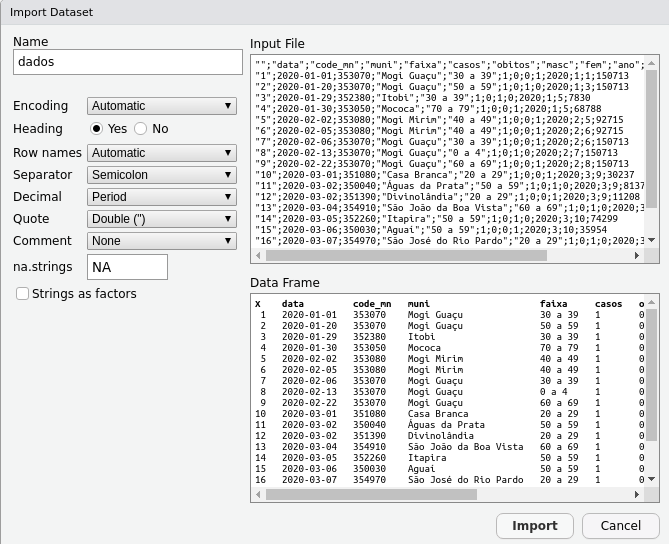
\includegraphics{ilustracoes/import_dataset.png}

\hypertarget{escrita-de-arquivos}{%
\section{Escrita de arquivos}\label{escrita-de-arquivos}}

\hypertarget{utilswrite.csv2}{%
\subsection{utils::write.csv2()}\label{utilswrite.csv2}}

É possível salvar um arquivo de dados que foi trabalhado no R em diferentes formatos, no caso, separado por ponto e vírgula. Um ponto negativo é que essa função, ao salvar o arquivo, cria uma coluna com nomes das linhas (em números).

\textbf{Exemplo}

\begin{Shaded}
\begin{Highlighting}[]
\FunctionTok{write.csv2}\NormalTok{(}\AttributeTok{x =}\NormalTok{ iris,                }\CommentTok{\# Dados ativos}
           \AttributeTok{file =} \StringTok{\textquotesingle{}dados/iris.csv\textquotesingle{}}\NormalTok{, }\CommentTok{\# Caminho e nome do arquivo}
           \AttributeTok{fileEncoding =} \StringTok{"UTF{-}8"}\NormalTok{)  }\CommentTok{\# Encoding}

\FunctionTok{read.csv2}\NormalTok{(}\StringTok{\textquotesingle{}dados/iris.csv\textquotesingle{}}\NormalTok{, }\AttributeTok{nrows =} \DecValTok{4}\NormalTok{)}
\end{Highlighting}
\end{Shaded}

\begin{verbatim}
##   X Sepal.Length Sepal.Width Petal.Length Petal.Width Species
## 1 1          5.1         3.5          1.4         0.2  setosa
## 2 2          4.9         3.0          1.4         0.2  setosa
## 3 3          4.7         3.2          1.3         0.2  setosa
## 4 4          4.6         3.1          1.5         0.2  setosa
\end{verbatim}

\textbf{Argumentos principais}

\begin{longtable}[]{@{}
  >{\raggedright\arraybackslash}p{(\columnwidth - 2\tabcolsep) * \real{0.5000}}
  >{\raggedright\arraybackslash}p{(\columnwidth - 2\tabcolsep) * \real{0.5000}}@{}}
\toprule
\begin{minipage}[b]{\linewidth}\raggedright
Argumento
\end{minipage} & \begin{minipage}[b]{\linewidth}\raggedright
Definição
\end{minipage} \\
\midrule
\endhead
x & Objeto a ser escrito, prefereincialmente uma matriz ou data.frame. \\
file & Nome do arquivo criado (pode conter o caminho) utilizando aspas '' ``. \\
append & Logical. Se TRUE os dados serão adicionados à última linha de um arquivo já existente, que deve ter o nome descrito em file, se FALSE qualquer arquivo com o nome descrito será sobrescrito. \\
na & String usada para valores ausentes nos dados. \\
dec & String para definir divisor de decimal, ex. dec = ``.''. \\
col.names & Logical. Indica se os nomes das colunas de x devem ser escritos junto com x, ou um vetor de caracteres dos nomes das colunas a serem escritos. \\
row.names & Logical. Cria coluna com nomes para linhas. \\
fileEncoding & String. Declara a codificação a ser usada para que possam ser recodificados à medida que são gravados. \\
\bottomrule
\end{longtable}

\hypertarget{readrwrite_csv2}{%
\subsection{readr::write\_csv2()}\label{readrwrite_csv2}}

É semelhante à função anterior, mas executa a tarefa duas vezes mais rápido, com a vantagem de não criar uma coluna com nomes das linhas.

\textbf{Exemplo}

\begin{Shaded}
\begin{Highlighting}[]
\NormalTok{readr}\SpecialCharTok{::}\FunctionTok{write\_csv2}\NormalTok{(}\AttributeTok{x =}\NormalTok{ iris, }\AttributeTok{file =} \StringTok{\textquotesingle{}dados/iris.csv\textquotesingle{}}\NormalTok{)}
\FunctionTok{read.csv2}\NormalTok{(}\AttributeTok{file =} \StringTok{\textquotesingle{}dados/iris.csv\textquotesingle{}}\NormalTok{, }\AttributeTok{nrows =} \DecValTok{4}\NormalTok{)}
\end{Highlighting}
\end{Shaded}

\begin{verbatim}
##   Sepal.Length Sepal.Width Petal.Length Petal.Width Species
## 1          5.1         3.5          1.4         0.2  setosa
## 2          4.9         3.0          1.4         0.2  setosa
## 3          4.7         3.2          1.3         0.2  setosa
## 4          4.6         3.1          1.5         0.2  setosa
\end{verbatim}

\textbf{Argumentos principais}
Argumento\textbar Definição
---------\textbar---------
x\\
A data frame or tibble to write to disk.

file\\
File or connection to write to.

delim\\
Delimiter used to separate values. Defaults to '' '' for write\_delim(), ``,'' for write\_excel\_csv() and ``;'' for write\_excel\_csv2(). Must be a single character.

na\\
String used for missing values. Defaults to NA. Missing values will never be quoted; strings with the same value as na will always be quoted.

append\\
If FALSE, will overwrite existing file. If TRUE, will append to existing file. In both cases, if the file does not exist a new file is created.

col\_names\\
If FALSE, column names will not be included at the top of the file. If TRUE, column names will be included. If not specified, col\_names will take the opposite value given to append.

quote\\
How to handle fields which contain characters that need to be quoted.

needed - Only quote fields which need them.

all - Quote all fields.

none - Never quote fields.

escape\\
The type of escape to use when quotes are in the data.

double - quotes are escaped by doubling them.

backslash - quotes are escaped by a preceding backslash.

none - quotes are not escaped.

eol

num\_threads
Number of threads to use when reading and materializing vectors. If your data contains newlines within fields the parser will automatically be forced to use a single thread only.

progress\\
Display a progress bar? By default it will only display in an interactive session and not while knitting a document. The display is updated every 50,000 values and will only display if estimated reading time is 5 seconds or more. The automatic progress bar can be disabled by setting option readr.show\_progress to FALSE.

\hypertarget{writexlwrite_xlsx}{%
\subsection{writexl::write\_xlsx()}\label{writexlwrite_xlsx}}

Salvar arquivo de dados como Excel, formato .xlsx.

\textbf{Exemplo 1}

\begin{Shaded}
\begin{Highlighting}[]
\NormalTok{writexl}\SpecialCharTok{::}\FunctionTok{write\_xlsx}\NormalTok{(}\AttributeTok{x =}\NormalTok{ iris,}
                    \AttributeTok{path =} \StringTok{\textquotesingle{}dados/iris.xlsx\textquotesingle{}}\NormalTok{,}
                    \AttributeTok{col\_names =} \ConstantTok{TRUE}\NormalTok{,}
                    \AttributeTok{format\_headers =} \ConstantTok{TRUE}\NormalTok{)}
\NormalTok{readxl}\SpecialCharTok{::}\FunctionTok{read\_excel}\NormalTok{(}\StringTok{\textquotesingle{}dados/iris.xlsx\textquotesingle{}}\NormalTok{, }\AttributeTok{n\_max =} \DecValTok{4}\NormalTok{)}
\end{Highlighting}
\end{Shaded}

\begin{verbatim}
## # A tibble: 4 x 5
##   Sepal.Length Sepal.Width Petal.Length Petal.Width Species
##          <dbl>       <dbl>        <dbl>       <dbl> <chr>  
## 1          5.1         3.5          1.4         0.2 setosa 
## 2          4.9         3            1.4         0.2 setosa 
## 3          4.7         3.2          1.3         0.2 setosa 
## 4          4.6         3.1          1.5         0.2 setosa
\end{verbatim}

\textbf{Exemplo 2}

\begin{Shaded}
\begin{Highlighting}[]
\NormalTok{writexl}\SpecialCharTok{::}\FunctionTok{write\_xlsx}\NormalTok{(}\AttributeTok{path =} \StringTok{"dados/conjuntodadosnativos.xlsx"}\NormalTok{,}
           \AttributeTok{x =} \FunctionTok{list}\NormalTok{(}\AttributeTok{sheet1=}\NormalTok{iris, }\AttributeTok{sheet2=}\NormalTok{cars, }\AttributeTok{sheet3=}\NormalTok{mtcars))}

\NormalTok{readxl}\SpecialCharTok{::}\FunctionTok{read\_excel}\NormalTok{(}\AttributeTok{path =} \StringTok{\textquotesingle{}dados/conjuntodadosnativos.xlsx\textquotesingle{}}\NormalTok{,}
                   \AttributeTok{sheet =} \DecValTok{3}\NormalTok{, }
                   \AttributeTok{n\_max =} \DecValTok{4}\NormalTok{)}
\end{Highlighting}
\end{Shaded}

\begin{verbatim}
## # A tibble: 4 x 11
##     mpg   cyl  disp    hp  drat    wt  qsec    vs    am  gear  carb
##   <dbl> <dbl> <dbl> <dbl> <dbl> <dbl> <dbl> <dbl> <dbl> <dbl> <dbl>
## 1  21       6   160   110  3.9   2.62  16.5     0     1     4     4
## 2  21       6   160   110  3.9   2.88  17.0     0     1     4     4
## 3  22.8     4   108    93  3.85  2.32  18.6     1     1     4     1
## 4  21.4     6   258   110  3.08  3.22  19.4     1     0     3     1
\end{verbatim}

\textbf{Argumentos principais}

\begin{longtable}[]{@{}
  >{\raggedright\arraybackslash}p{(\columnwidth - 2\tabcolsep) * \real{0.5000}}
  >{\raggedright\arraybackslash}p{(\columnwidth - 2\tabcolsep) * \real{0.5000}}@{}}
\toprule
\begin{minipage}[b]{\linewidth}\raggedright
Argumento
\end{minipage} & \begin{minipage}[b]{\linewidth}\raggedright
Definição
\end{minipage} \\
\midrule
\endhead
x & Data frame ou lista de data frames que serão salvos em planilhas (sheets). \\
path & Nome do arquuivo criado. \\
col\_names & Se TRUE, primera linha traz os nomes das colunas. \\
format\_headers & Inserir nomes das colunas. \\
\bottomrule
\end{longtable}

\hypertarget{data.tablefwrite}{%
\subsection{data.table::fwrite()}\label{data.tablefwrite}}

\hypertarget{cross}{%
\chapter{Cross-references}\label{cross}}

Cross-references make it easier for your readers to find and link to elements in your book.

\hypertarget{chapters-and-sub-chapters}{%
\section{Chapters and sub-chapters}\label{chapters-and-sub-chapters}}

There are two steps to cross-reference any heading:

\begin{enumerate}
\def\labelenumi{\arabic{enumi}.}
\tightlist
\item
  Label the heading: \texttt{\#\ Hello\ world\ \{\#nice-label\}}.

  \begin{itemize}
  \tightlist
  \item
    Leave the label off if you like the automated heading generated based on your heading title: for example, \texttt{\#\ Hello\ world} = \texttt{\#\ Hello\ world\ \{\#hello-world\}}.
  \item
    To label an un-numbered heading, use: \texttt{\#\ Hello\ world\ \{-\#nice-label\}} or \texttt{\{\#\ Hello\ world\ .unnumbered\}}.
  \end{itemize}
\item
  Next, reference the labeled heading anywhere in the text using \texttt{\textbackslash{}@ref(nice-label)}; for example, please see Chapter \ref{cross}.

  \begin{itemize}
  \tightlist
  \item
    If you prefer text as the link instead of a numbered reference use: \protect\hyperlink{cross}{any text you want can go here}.
  \end{itemize}
\end{enumerate}

\hypertarget{captioned-figures-and-tables}{%
\section{Captioned figures and tables}\label{captioned-figures-and-tables}}

Figures and tables \emph{with captions} can also be cross-referenced from elsewhere in your book using \texttt{\textbackslash{}@ref(fig:chunk-label)} and \texttt{\textbackslash{}@ref(tab:chunk-label)}, respectively.

See Figure \ref{fig:nice-fig}.

\begin{Shaded}
\begin{Highlighting}[]
\FunctionTok{par}\NormalTok{(}\AttributeTok{mar =} \FunctionTok{c}\NormalTok{(}\DecValTok{4}\NormalTok{, }\DecValTok{4}\NormalTok{, .}\DecValTok{1}\NormalTok{, .}\DecValTok{1}\NormalTok{))}
\FunctionTok{plot}\NormalTok{(pressure, }\AttributeTok{type =} \StringTok{\textquotesingle{}b\textquotesingle{}}\NormalTok{, }\AttributeTok{pch =} \DecValTok{19}\NormalTok{)}
\end{Highlighting}
\end{Shaded}

\begin{figure}

{\centering 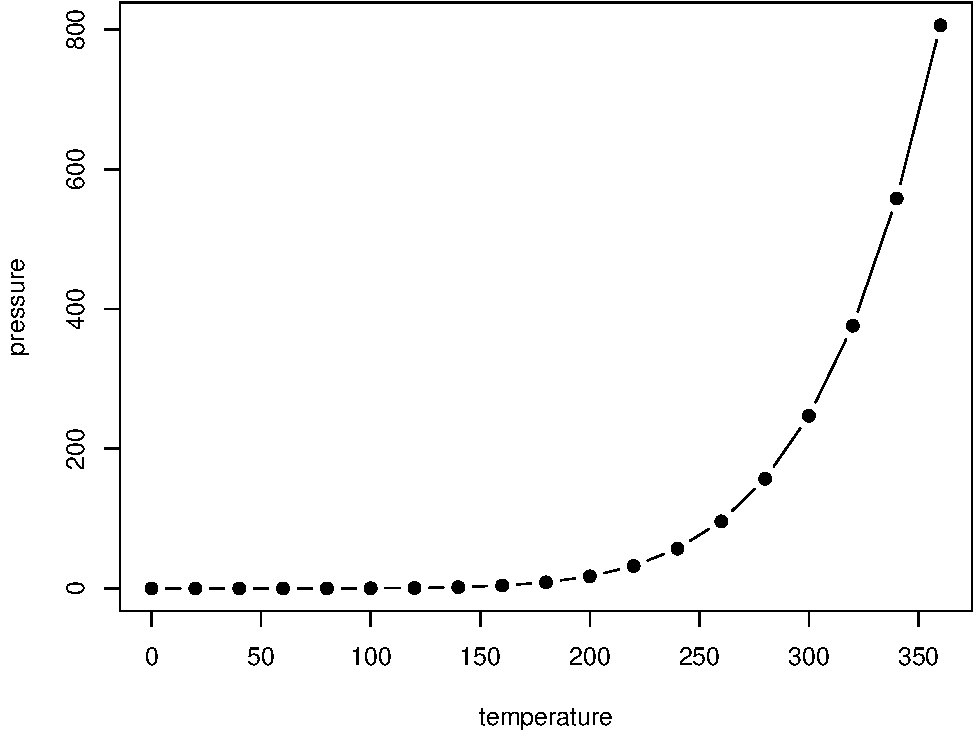
\includegraphics[width=0.8\linewidth]{guia_bolso_R_files/figure-latex/nice-fig-1} 

}

\caption{Here is a nice figure!}\label{fig:nice-fig}
\end{figure}

Don't miss Table \ref{tab:nice-tab}.

\begin{Shaded}
\begin{Highlighting}[]
\NormalTok{knitr}\SpecialCharTok{::}\FunctionTok{kable}\NormalTok{(}
  \FunctionTok{head}\NormalTok{(pressure, }\DecValTok{10}\NormalTok{), }\AttributeTok{caption =} \StringTok{\textquotesingle{}Here is a nice table!\textquotesingle{}}\NormalTok{,}
  \AttributeTok{booktabs =} \ConstantTok{TRUE}
\NormalTok{)}
\end{Highlighting}
\end{Shaded}

\begin{table}

\caption{\label{tab:nice-tab}Here is a nice table!}
\centering
\begin{tabular}[t]{rr}
\toprule
temperature & pressure\\
\midrule
0 & 0.0002\\
20 & 0.0012\\
40 & 0.0060\\
60 & 0.0300\\
80 & 0.0900\\
\addlinespace
100 & 0.2700\\
120 & 0.7500\\
140 & 1.8500\\
160 & 4.2000\\
180 & 8.8000\\
\bottomrule
\end{tabular}
\end{table}

\hypertarget{parts}{%
\chapter{Parts}\label{parts}}

You can add parts to organize one or more book chapters together. Parts can be inserted at the top of an .Rmd file, before the first-level chapter heading in that same file.

Add a numbered part: \texttt{\#\ (PART)\ Act\ one\ \{-\}} (followed by \texttt{\#\ A\ chapter})

Add an unnumbered part: \texttt{\#\ (PART\textbackslash{}*)\ Act\ one\ \{-\}} (followed by \texttt{\#\ A\ chapter})

Add an appendix as a special kind of un-numbered part: \texttt{\#\ (APPENDIX)\ Other\ stuff\ \{-\}} (followed by \texttt{\#\ A\ chapter}). Chapters in an appendix are prepended with letters instead of numbers.

\hypertarget{footnotes-and-citations}{%
\chapter{Footnotes and citations}\label{footnotes-and-citations}}

\hypertarget{footnotes}{%
\section{Footnotes}\label{footnotes}}

Footnotes are put inside the square brackets after a caret \texttt{\^{}{[}{]}}. Like this one \footnote{This is a footnote.}.

\hypertarget{citations}{%
\section{Citations}\label{citations}}

Reference items in your bibliography file(s) using \texttt{@key}.

For example, we are using the \textbf{bookdown} package \citep{R-bookdown} (check out the last code chunk in index.Rmd to see how this citation key was added) in this sample book, which was built on top of R Markdown and \textbf{knitr} \citep{xie2015} (this citation was added manually in an external file book.bib).
Note that the \texttt{.bib} files need to be listed in the index.Rmd with the YAML \texttt{bibliography} key.

The RStudio Visual Markdown Editor can also make it easier to insert citations: \url{https://rstudio.github.io/visual-markdown-editing/\#/citations}

\hypertarget{blocks}{%
\chapter{Blocks}\label{blocks}}

\hypertarget{equations}{%
\section{Equations}\label{equations}}

Here is an equation.

\begin{equation} 
  f\left(k\right) = \binom{n}{k} p^k\left(1-p\right)^{n-k}
  \label{eq:binom}
\end{equation}

You may refer to using \texttt{\textbackslash{}@ref(eq:binom)}, like see Equation \eqref{eq:binom}.

\hypertarget{theorems-and-proofs}{%
\section{Theorems and proofs}\label{theorems-and-proofs}}

Labeled theorems can be referenced in text using \texttt{\textbackslash{}@ref(thm:tri)}, for example, check out this smart theorem \ref{thm:tri}.

\begin{theorem}
\protect\hypertarget{thm:tri}{}\label{thm:tri}For a right triangle, if \(c\) denotes the \emph{length} of the hypotenuse
and \(a\) and \(b\) denote the lengths of the \textbf{other} two sides, we have
\[a^2 + b^2 = c^2\]
\end{theorem}

Read more here \url{https://bookdown.org/yihui/bookdown/markdown-extensions-by-bookdown.html}.

\hypertarget{callout-blocks}{%
\section{Callout blocks}\label{callout-blocks}}

The R Markdown Cookbook provides more help on how to use custom blocks to design your own callouts: \url{https://bookdown.org/yihui/rmarkdown-cookbook/custom-blocks.html}

\hypertarget{sharing-your-book}{%
\chapter{Sharing your book}\label{sharing-your-book}}

\hypertarget{publishing}{%
\section{Publishing}\label{publishing}}

HTML books can be published online, see: \url{https://bookdown.org/yihui/bookdown/publishing.html}

\hypertarget{pages}{%
\section{404 pages}\label{pages}}

By default, users will be directed to a 404 page if they try to access a webpage that cannot be found. If you'd like to customize your 404 page instead of using the default, you may add either a \texttt{\_404.Rmd} or \texttt{\_404.md} file to your project root and use code and/or Markdown syntax.

\hypertarget{metadata-for-sharing}{%
\section{Metadata for sharing}\label{metadata-for-sharing}}

Bookdown HTML books will provide HTML metadata for social sharing on platforms like Twitter, Facebook, and LinkedIn, using information you provide in the \texttt{index.Rmd} YAML. To setup, set the \texttt{url} for your book and the path to your \texttt{cover-image} file. Your book's \texttt{title} and \texttt{description} are also used.

This \texttt{gitbook} uses the same social sharing data across all chapters in your book- all links shared will look the same.

Specify your book's source repository on GitHub using the \texttt{edit} key under the configuration options in the \texttt{\_output.yml} file, which allows users to suggest an edit by linking to a chapter's source file.

Read more about the features of this output format here:

\url{https://pkgs.rstudio.com/bookdown/reference/gitbook.html}

Or use:

\begin{Shaded}
\begin{Highlighting}[]
\NormalTok{?bookdown}\SpecialCharTok{::}\NormalTok{gitbook}
\end{Highlighting}
\end{Shaded}


  \bibliography{book.bib,packages.bib}

\end{document}
